\section{Verteilung der Anwendung}
\label{subsec:implementation:ApplicationDistribution}
Eine wesentliche Anforderung an die Praxisanwendung ist, dem Anforderungskatalog unter Kapitel \ref{sec:Eruierung:technicalRequierements} entsprechend, die Fokussierung der Softwarearchitektur auf die auf Verteilung der gesamten Anwendung. Dies kann erreicht werden, indem die Anwendung in verschiedene Services unterteilt wird, siehe dazu in Abschnitt \ref{sec:implementation:serviceAndComponentOrientation}. \\
Für die Erstellung von Instanzen dieser Komponenten wurden vier verschiedene Konsolenanwendungen implementiert, wobei für jeden Service ein eigene Anwendung geschrieben wurde. Eine Ausnahme stellen hier \textit{Domain-Service} und \textit{Command-Service} dar, denn sie operieren in einer gemeinsamen Anwendung. \\
Die Verbindung zwischen den einzelnen Komponenten wird mit der Cluster-Unterstützung umgesetzt, welche \textit{Akka.net} mitliefert und im nachfolgenden Abschnitt \ref{subsec:implementation:akka:cluster} beschrieben ist. 

\subsection{Cluster}
\label{subsec:implementation:akka:cluster}
Die Cluster-Funktionalität von \textit{Akka.net} bietet die Möglichkeit, zusammengehörende Anwendungen über ein Netzwerk zu verbinden und somit einen Cluster zu formen. Für den Benutzer der Anwendung harmoniert der Cluster als eine geschlossene Einheit. Dazu werden mittels einem \textit{Peer-to-Peer} Netzwerk alle teilnehmenden Anwendungen untereinander verbunden. Über ein Protokoll, das sogenannte \textit{Gossip}, genauer beschrieben in Abschnitt \ref{subsec:implementation:gossip}, werden Informationen zum Zustand des Clusters ausgetauscht. Jede am Cluster teilnehmende Anwendung wird als Node bezeichnet. Somit bilden zwei oder mehr Nodes einen Cluster \citep{akkaInAction}. \\
Jede Anwendung bekommt Rollen zugewissen, welche es zur Laufzeit übernehmen kann. Eine Rolle definiert in \textit{Akka.net} ein Aufgabengebiet innerhalb des Clusters. Für \textit{TyrolSky} wurden die fünf, in Abschnitt \ref{sec:implementation:serviceAndComponentOrientation}definierten, Services als Rollen herangenommen. Tritt eine Anwendung dem Cluster bei, so gibt sie während dem Eintrittverfahren bekannt, welche Rollen sie im Cluster übernehmen kann. Eine Rolle kann somit mehrfach im Cluster vorhanden und mehrfach redundant ausgelegt sein. \\
Die Kommunikation zwischen den Komponenten erfolgt innerhalb des \textit{Akka.net} Cluster entweder über Routing-Mechanismen, siehe Abschnitt \ref{subsec:implementation:akkaRouting}, oder über verteilte Daten, welche in \textit{Shards} organisiert sind, nachzulesen in Abschnitt \ref{subsec:implementation:akkaSharding}. 

\subsection{Routing}
\label{subsec:implementation:akkaRouting}
In Kapitel \ref{sec:actor:patterns:routing} wurde darauf eingegangen, dass es in einem System Actors geben kann, welche für die Verteilung von Nachrichten an verschiedene Actors zuständig sind. Die Verteilung von Nachrichten zwischen den teilnehmenden Nodes, in einem auf \textit{Akka.net} Cluster aufbauenden System, wird durch eben solche Router bewerkstelligt \citep{Akka.netCommunityAkka.NETDocumentation}. \\
Das Framework bietet dabei verschiedene Typen von Actors an, die Nachrichten annehmen und an andere Actors, auf entfernten Nodes, weiterleiten. Die auf das Weiterleiten von Nachrichten spezialisierte Actoren werden Router genannt. Bei der Erstellung eines Routers wird über Parameter angegeben, welche Actoren als Ziel dienen können und welche Routingsstrategie verwendet werden soll. Möglichen Rollen, auf denen sich die Ziele befinden, können eingeschränkt werden. Nachfolgend wird die verwendeten Routingsstrategie innerhalb von \textit{TyrolSky} beschrieben. \\
Sämtliche Anfragen an das System haben ihren Startpunkt bei der Komponente \textit{API-Service}. Von dieser müssen Anfragen an die betreffenden Komponenten weitergeleitet werden. Die entsprechende Komponente kann sich, da die Anwendung mit dem \textit{CQRS}-Prinzip arbeitet, nur in den Rollen \textit{Command-Service} und \textit{Query-Service} befinden. Bei einer ankommenden Anfrage kann der \textit{API-Service} aufgrund des Types der Anfrage entscheiden, ob die weitere Verarbeitung in einem \textit{Query} oder \textit{Command-Service} stattfinden soll. Dementsprechend wird die Anfrage an den Router, welcher für den entsprechenden Service zuständig ist, weitergeleitet. Der Router überwacht mithilfe von Informationen, welche er über \textit{Gossip} erhält, den Status von anderen Nodes mit der entsprechenden Rolle im Cluster. Empfängt der Router eine Nachricht, so kann er eine der in Frage kommenden, verfügbaren Nodes auswählen und die Nachricht an diesen zustellen. \\
Bei der Auswahl des entsprechenden Zielnodes wird für den Router das \textit{Round-Robin} Verfahren eingesetzt. Somit ist eine gleichmäßige Verteilung der Nachrichten auf unterschiedliche Hosts möglich. Es gibt neben dem \textit{Round-Robin} Routingverfahren noch andere bereits implementierte Routingsstrategien innerhalb von \text{Akka.net}. Unter anderem werden die Strategien zufälliges Routing, Hashingrouting oder kleinste Mailbox vom Framework mitgeliefert \citep{Akka.netCommunityAkka.NETDocumentation}. Jedoch werden diese im Zuge der Umsetzung von \textit{TyrolSky} nicht verwendet. \\
In Abbildung \ref{fig:implementation:routing} ist das Zusammenspiel der drei Komponenten \textit{API-Service}, \textit{Query-Service} und \textit{Command-Service} zu sehen, wobei von den zwei zuletzt genannten jeweils zwei Instanzen am Cluster teilnehmen. Die Router auf dem Node \textit{A} leiten die Nachrichten abwechselnd an die zwei Nodes \textit{B} und \textit{C} oder an \textit{D} und \textit{E} weiter. 

\begin{figure}
  \centering
  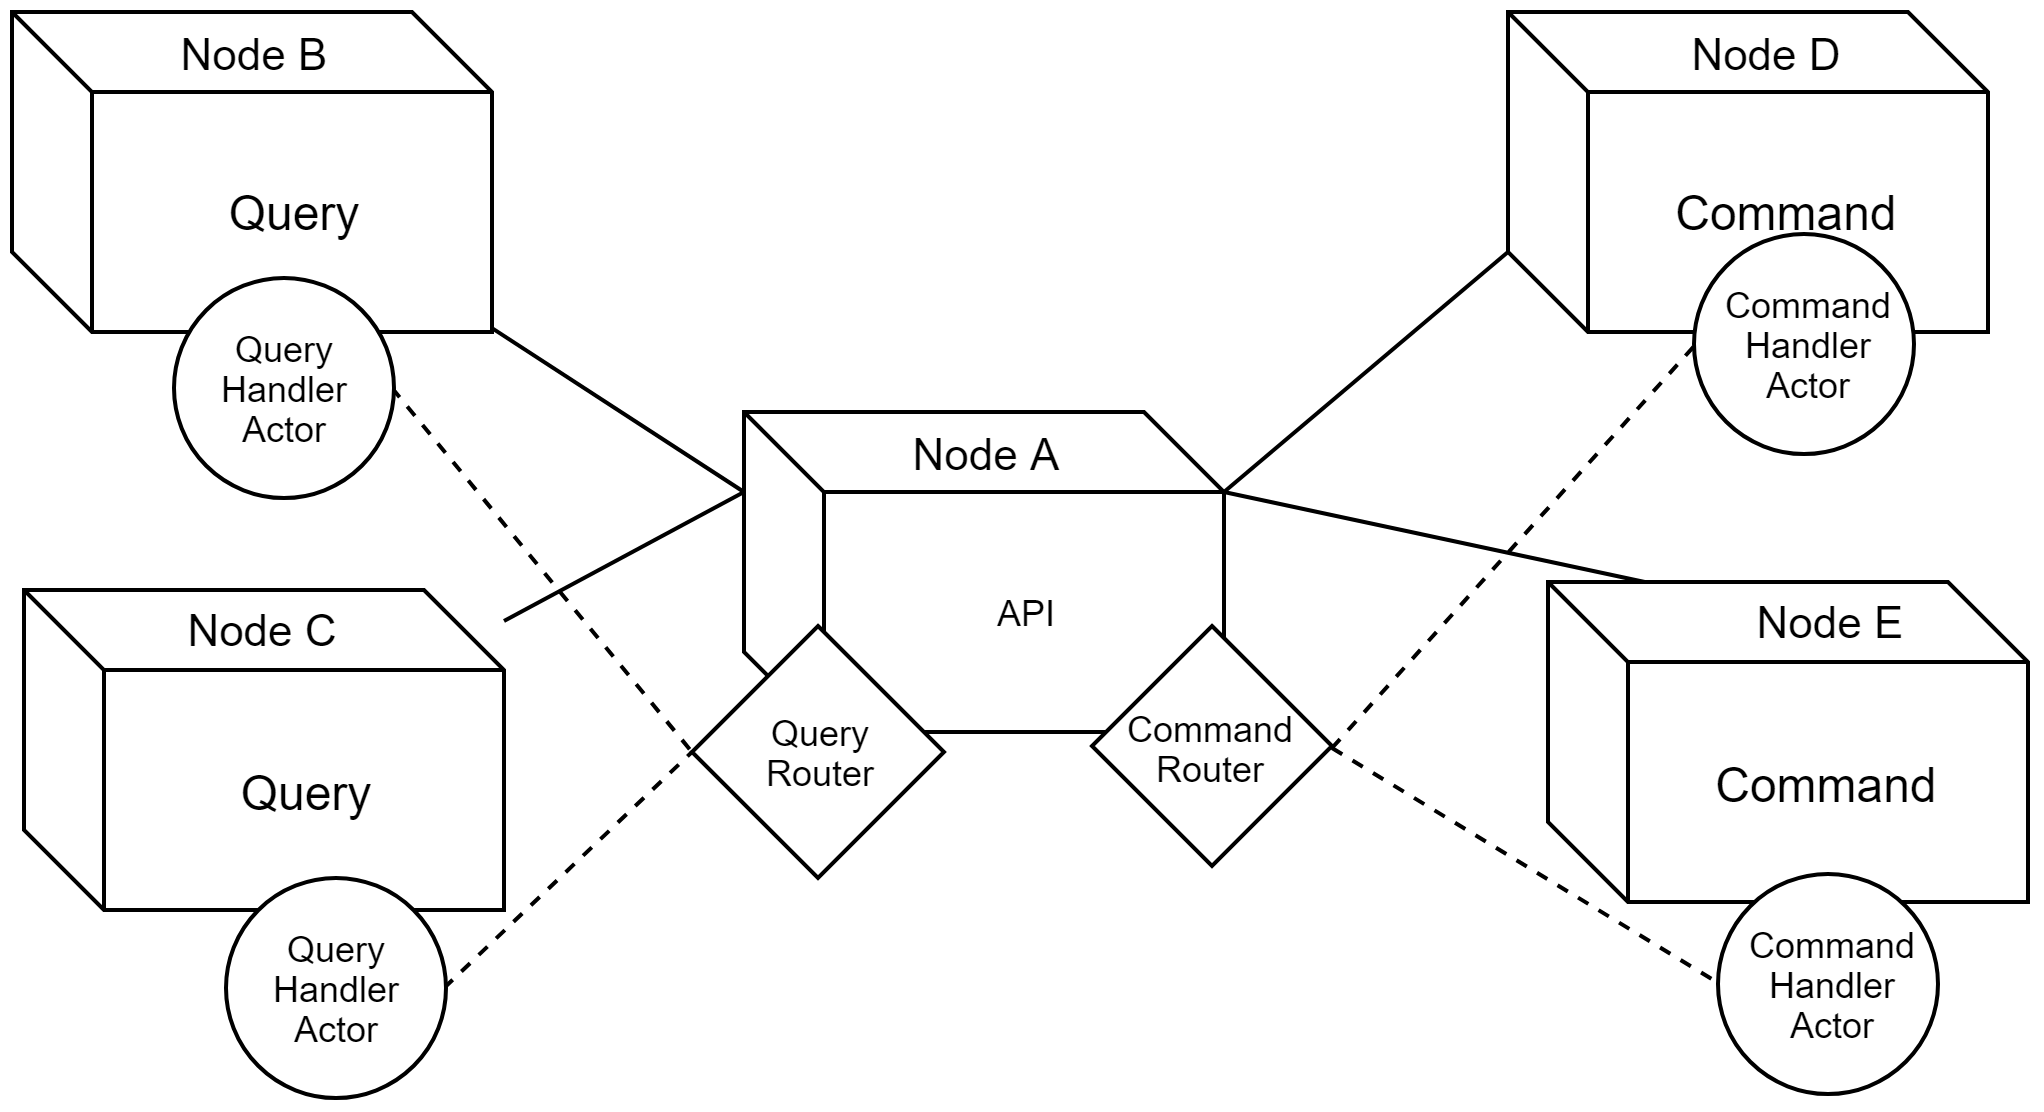
\includegraphics[width=\linewidth]{gfx/implementation/ClusterRouter}
  \caption{Ein \textit{Round-Robin} Router, welcher Nachrichten von der Komponente \textit{API} auf andere Komponenten verteilt.}
  \label{fig:implementation:routing}
\end{figure} 

\subsection{Gossip}
\label{subsec:implementation:gossip}
Bereits in Abschnitt \ref{subsec:implementation:lighthouse} wurde die Komponente \textit{Lighthouse} vorgestellt, welche als Einstiegspunkt für alle teilnehmenden Nodes verwendet wird. Die Verbindung zu den restlichen, im Cluster vorhandenen Nodes wird über das \textit{Gossip}-Protokoll hergestellt. \\
Gossip kommt aus dem Englischen, und beschreibt Klatsch-Gespräche innerhalb einer sozialen Gruppe. 
In dem Cluster-Protokoll Akka-\textit{Gossip} wird diese Art der Kommunikation angewendet, indem Nodes Änderungen am Clusterzustand ihren Nachbarn mitteilen \citep{Akka.netCommunityAkka.NETDocumentation}. \\
Nodes mit der Rolle \textit{Lighthouse} sind der Start dieser Kommunikation. Deshalb müssen diese Nodes auch über eine fixe Adresse verfügen, im Fall von \textit{TyrolSky} sind das Ip-Adresse sowie Port. Komponenten welche nun dem Cluster beitreten wollen, melden sich bei einem der \textit{Lighthouse}-Komponenten an und geben bekannt, über welche Adresse sie erreichbar sind. Über das \textit{Gossip}-Protokoll wird nun jedem bereits im System beigetretenen Node mitgeteilt, dass sich ein neuer Node im Cluster befindet. \\
In der Kommunikation zwischen den Nodes wird jedem einzelnen mitgeteilt, welche Rollen eine teilnehmende Instanz besitzt. Dies wird dann anschließend von den Routern, siehe Abschnitt \ref{fig:implementation:routing}, verwendet, um Nachrichten an diese Rolle zuzustellen. Das Protokoll beinhaltet auch Informationen über den aktuellen Zustand der einzelnen Nodes. So werden beispielsweise alle Nodes über eine fehlerhafte Verbindung zwischen zwei einzelnen Nodes benachrichtigt. Ist ein Node nicht mehr erreichbar, ohne dass eine kontrollierte Abmeldung vom Cluster stattgefunden hat, kann er nicht einfach aus dem Cluster entfernt werden. Um den fehlerhaften Zustand des Clusters zu lösen, soll eine Lösungsstrategie implementiert werden, welche wieder einen fehlerfreien Zustand herstellt, siehe dazu den nachfolgenden Abschnitt \ref{subsec:implementation:splitBrain}. \\ 
Das \textit{Gossip}-Protokoll dient, neben der Zusammenfügung der einzelnen Node zu einem Cluster, auch zum Austausch von Informationen über den aktuellen Zustand der einzelnen Nodes. Muss vom Protokoll eine Entscheidung getroffen werden, wie beispielsweise die Entscheidung, ob ein neuer Node dem Cluster beitreten darf, wird ein dafür definierter Node benötigt, welcher diese Entscheidungen treffen kann. Im Fall von \textit{TyrolSky} ist das immer der ältester Node im Cluster. Wird dieser vom Cluster entfernt, übernimmt die Führung der nächst älteste im Cluster enthaltende Node. Über diesen, in \textit{Akka.net} bezeichneten \textit{Leader}, werden Entscheidungen getroffen, welche für \textit{Gossip} relevant sind \citep{akkaInAction}. 

\subsection{Split-Brain} 
\label{subsec:implementation:splitBrain}
Wie bereits in Kapitel \ref{sec:distributedSystems:capTheorem} besprochen, kann bei einer Verbindung zwischen zwei Geräten jederzeit ein Problem auftreten, das die Kommunikation zwischen den Teilnehmern stört oder gänzlich unterbricht. Bei einer solchen Störung ist es dem betroffenen Node nicht mehr möglich, am \textit{Gossip} teilzunehmen und seinen Zustand anderen mitzuteilen. Auch wissen anderen Cluster Teilnehmer den Grund für Trennung der Kommunikation nicht. Deshalb können diese keine Aussage treffen, ob die Trennung des Teilnehmers nur temporär ist oder ob der Partner gar nicht mehr existiert. \\
Ein ähnliches Szenario kann auch auftreten, wenn zwei oder mehr Gruppen von Nodes zwar untereinander eine aufrechte Kommunikation führen, jedoch die Gruppen selbst voneinander getrennt wurden. So agiert jede Gruppe des Clusters für sich selber und kann sich mit den anderen Gruppen nicht mehr verständigen. Würde nun jeder Node im Cluster andere Nodes, welche für ihn nicht erreichbar sind, selbstständig entfernen, so würde jede Gruppe einen eigenen, neuen Cluster bilden, was als \textit{Split-Brain} bezeichnet wird \citep{networkIsReliable}. Bildet sich aus einem Cluster, durch gegenseitiges Entfernen, mehrere neue Clusters, so entstehen dadurch zwei oder mehrere Parallelstrukturen, welche die Konsistenz der gesamten Applikation verletzen können. Unter anderem werden die Prinzipien von \textit{Cluster Singletons} oder \textit{Sharding} verletzt und dies kann entsprechend zu Redundanzen führen. \\
In \textit{Akka.net} gibt es einige Strategieren, welche für das \textit{Split-Brain} Problem angewandt wurden. Jede Strategie hat jedoch einen Nachteil der teilweise sogar zum Stillstand der gesamten Anwendung führen kann. Nachfolgend die, laut \cite{Akka.netCommunityAkka.NETDocumentation} bereits verfügbaren, Strategien mit ihren Vor- und Nachteilen die durch dasFramework zur Verfügung stehen.
\begin{itemize}
  \litem{Statische Mehrheit}
  Jedem teilnehmenden Node wird die gleiche statische Nummer beim Start übergeben. Kann ein Node weniger Teilnehmer erreichen als die Nummer angibt, so beendet sich der Node selbstständig. Dadurch werden kleine gesplittete Gruppen automatisch beendet. Teilt sich jedoch das Netzwerk in mehr als zwei Gruppen auf, werden alle Nodes im gesamten Netzwerk beendet. 
  \litem{Behalte Mehrheit}
  Wird der Cluster durch ein Netzwerkproblem geteilt, wird anhand der zuletzt verfügbaren Informationen über den gesamten Cluster analysiert, ob der nun erreichbare Teil des Clusters die Mehrheit der vor der Unterbrechung beteiligten Nodes erreichen kann. Entspricht der neue Cluster der Mehrheit, werden die Nodes aufrechterhalten, anderenfalls werden alle Nodes des gesplitteten Clusters beendet. Auch hier kann das Aufteilen des Clusters in mehr als zwei Gruppen zum Stillstand des gesamten Clusters führen.
  \litem{Behalte Älteste}
  Durch das \textit{Gossip Protokoll}, siehe Abschnitt \ref{subsec:implementation:gossip}, wird mitgeteilt, zu welchem Zeitpunkt ein Node dem Cluster beigetreten ist. Darauf basierend kann berechnet werden, welcher Node der älteste im Cluster ist. Sobald sich der Cluster aufteilt, werden alle Nodes beendet, die den ältesten Node nicht erreichen können. Dadurch ist sichergestellt, das auch bei einer mehrfachen Aufteilung nicht der ganze Cluster beendet wird. Wird der Teil vom Node getrennt, der den ältesten Nodes und einige wenige andere Cluster beinhalteten, wird der gesamte größere Teil des Clusters beendet. Die Anwendung ist zwar nicht beendet, jedoch wurden mehr Nodes beendet als nötig. 
  \litem{Behalte Referenz}  
  Es wird ein fixer Nodes bestimmt, der für jeden Node erreichbar sein muss. Wird dieser von einem einzelnen nicht mehr erreicht, so wird dieser automatisch beendet. Dies führt dazu, dass wenn der referenzierte Node im gesamten Cluster nicht mehr erreichbar ist, die gesamte Anwendung beendet wird. Jedoch ist eine Aufteilung in zwei Teilen, der sogenannte \textit{Split-Brain} nicht möglich.
\end{itemize}
Für die Implementierung der \textit{TyrolSky} Anwendung wurde die Strategie \textit{Behalte Älteste} gewählt. Eine Zersplitterung des Clusters ist somit äußerst unwahrscheinlich. Das Risiko zu viele Nodes im Fehlerzustand zu beenden und das System somit kurzfristig zu verlangsamen, wird eingegangen, um die Datenkonsistenz für das \textit{Sharding} nicht zu verletzen.  

\subsection{Globale Dienste}
\label{subsec:implementation:singeltons}
Bereits in Abschnitt \ref{subsubsub:implementation:queryActorModel:resultPreparator} wurde ein Actor benötigt der nur exakt einmal im gesamten Cluster instanziiert werden darf um korrekt zu funktionieren. Im konkreten Beispiel war dies erforderlich, da der Actor für andere Actoren eindeutige, wiederverwendbare Namen generieren muss. In \textit{Akka.net} werden solche Actoren als \textit{Singletons} bezeichnet. Das Framework gewährleistet, dass die Actors die als Singletons deklariert sind, nur einmal im Cluster vorhanden sein können. Dabei wird auch berücksichtigt, dass wenn der Node auf welchem der Singleton Actor läuft, vom Cluster entfernt wird, der Singleton-Actor auf einen anderen Node im Cluster verschoben wird. Dadurch ist der Actor, mit Ausnahme der Zeit die der Prozess des Verschiebens von Actoren benötigt, zu jederzeit im System exakt einmal verfügbar. \\
Für die Überwachung und das Management der einzelnen Singleton-Actors ist der führende Cluster Node zuständig, siehe dazu Abschnitt \ref{subsec:implementation:gossip}. Jedem Singleton kann auch eine Cluster Rolle zugewissen werden, anschließend werden diese Singletons nur auf Nodes, welche dieser Rolle zugeordnet sind, ausgerollt. \\
Für die Implementierung von \textit{TyrolSky} wurden zwei Singletons eingesetzt. Beide werden für die Umsetzung der Namenverwaltung für die beiden Ergebnissaufbereiter im \textit{Query Service} benötigt. Den zwei Singletons wurde die Rolle \textit{Query} zugewiesen, womit sie nur auf den Nodes laufen, auf welchem sich die Ergebnisaufbereiter befinden.

\subsection{Verteilung transaktionaler Daten}
\label{subsec:implementation:akkaSharding}
Ein wesentlicher Teil der Komponente \textit{Domain Service}, Abschnitt \ref{subsec:implementation:domainService}, ist das Verteilen der Entitäten auf verschiedene Nodes der Rolle \textit{Domain Service}. Die Verteilung der Entitäten über den gesamten Cluster wird mit dem Prinzip des \textit{Shardings} umgesetzt. \\
Die Idee hinter \textit{Sharding} basiert auf Vorgehensweisen für verteilte Datenbanken und bedeutet laut \cite{shardingCattell}, dass Daten mithilfe eines Schlüssels auf unterschiedliche Hosts verteilt werden. Dabei bekommt jeder beteiligte Host einen bestimmten Bereich der Schlüsselmenge zugeteilt.
Die Information welche Schlüsselbereiche welchem Host zugeordnet sind, wird von jedem einzelnen Host geführt. Dadurch kann der Host durch den Schlüssel selber feststellen wo sich die entsprechende Datei befindet.
Dadurch ist eine effektive Verteilung von Daten auf unterschiedliche Hosts möglich, ohne das dabei jeder Beteiligte sämtliche Daten besitzen muss. Jedoch soll für eine Abfrage immer der dazugehörige Schlüssel bekannt sein. \\
Die Implementierung von \textit{TyrolSky} benützt diese Technik, mithilfe von \textit{Akka.net}, um Actoren über mehrere Nodes zu verteilen und dabei sicherstellen, dass diese von jedem anderen Node erreicht werden können. Dazu werden die Entitäten, also die Actoren welche im Sharding Cluster leben sollen, in \textit{Shards} unterteilt. Auf jedem Node der \textit{Shards} übernehmen soll, wird ein oder mehrere \textit{Shard Regions} gestartet. Dieser übernimmt, wie in Abbildung \ref{fig:implementation:actorSharding} dargestellt, die im zugewiesenen \textit{Shards} und startet die darin befindlichen Entitäten. Die Anzahl an möglichen \text{Shards} wird darbei für eine Anwendung fixiert. Im Falle von \textit{TyrolSky} werden {100} \textit{Shards} verwendet. Diese werden gleichmäßig an die verfügbaren \textit{Shard Regions} verteilt. Wird eine neue Region hinzugefügt, erfolgt eine Umverteilung der \textit{Shards}, womit auch die darin befindlichen Actors umverteilt werden. 

\begin{figure}
  \centering
  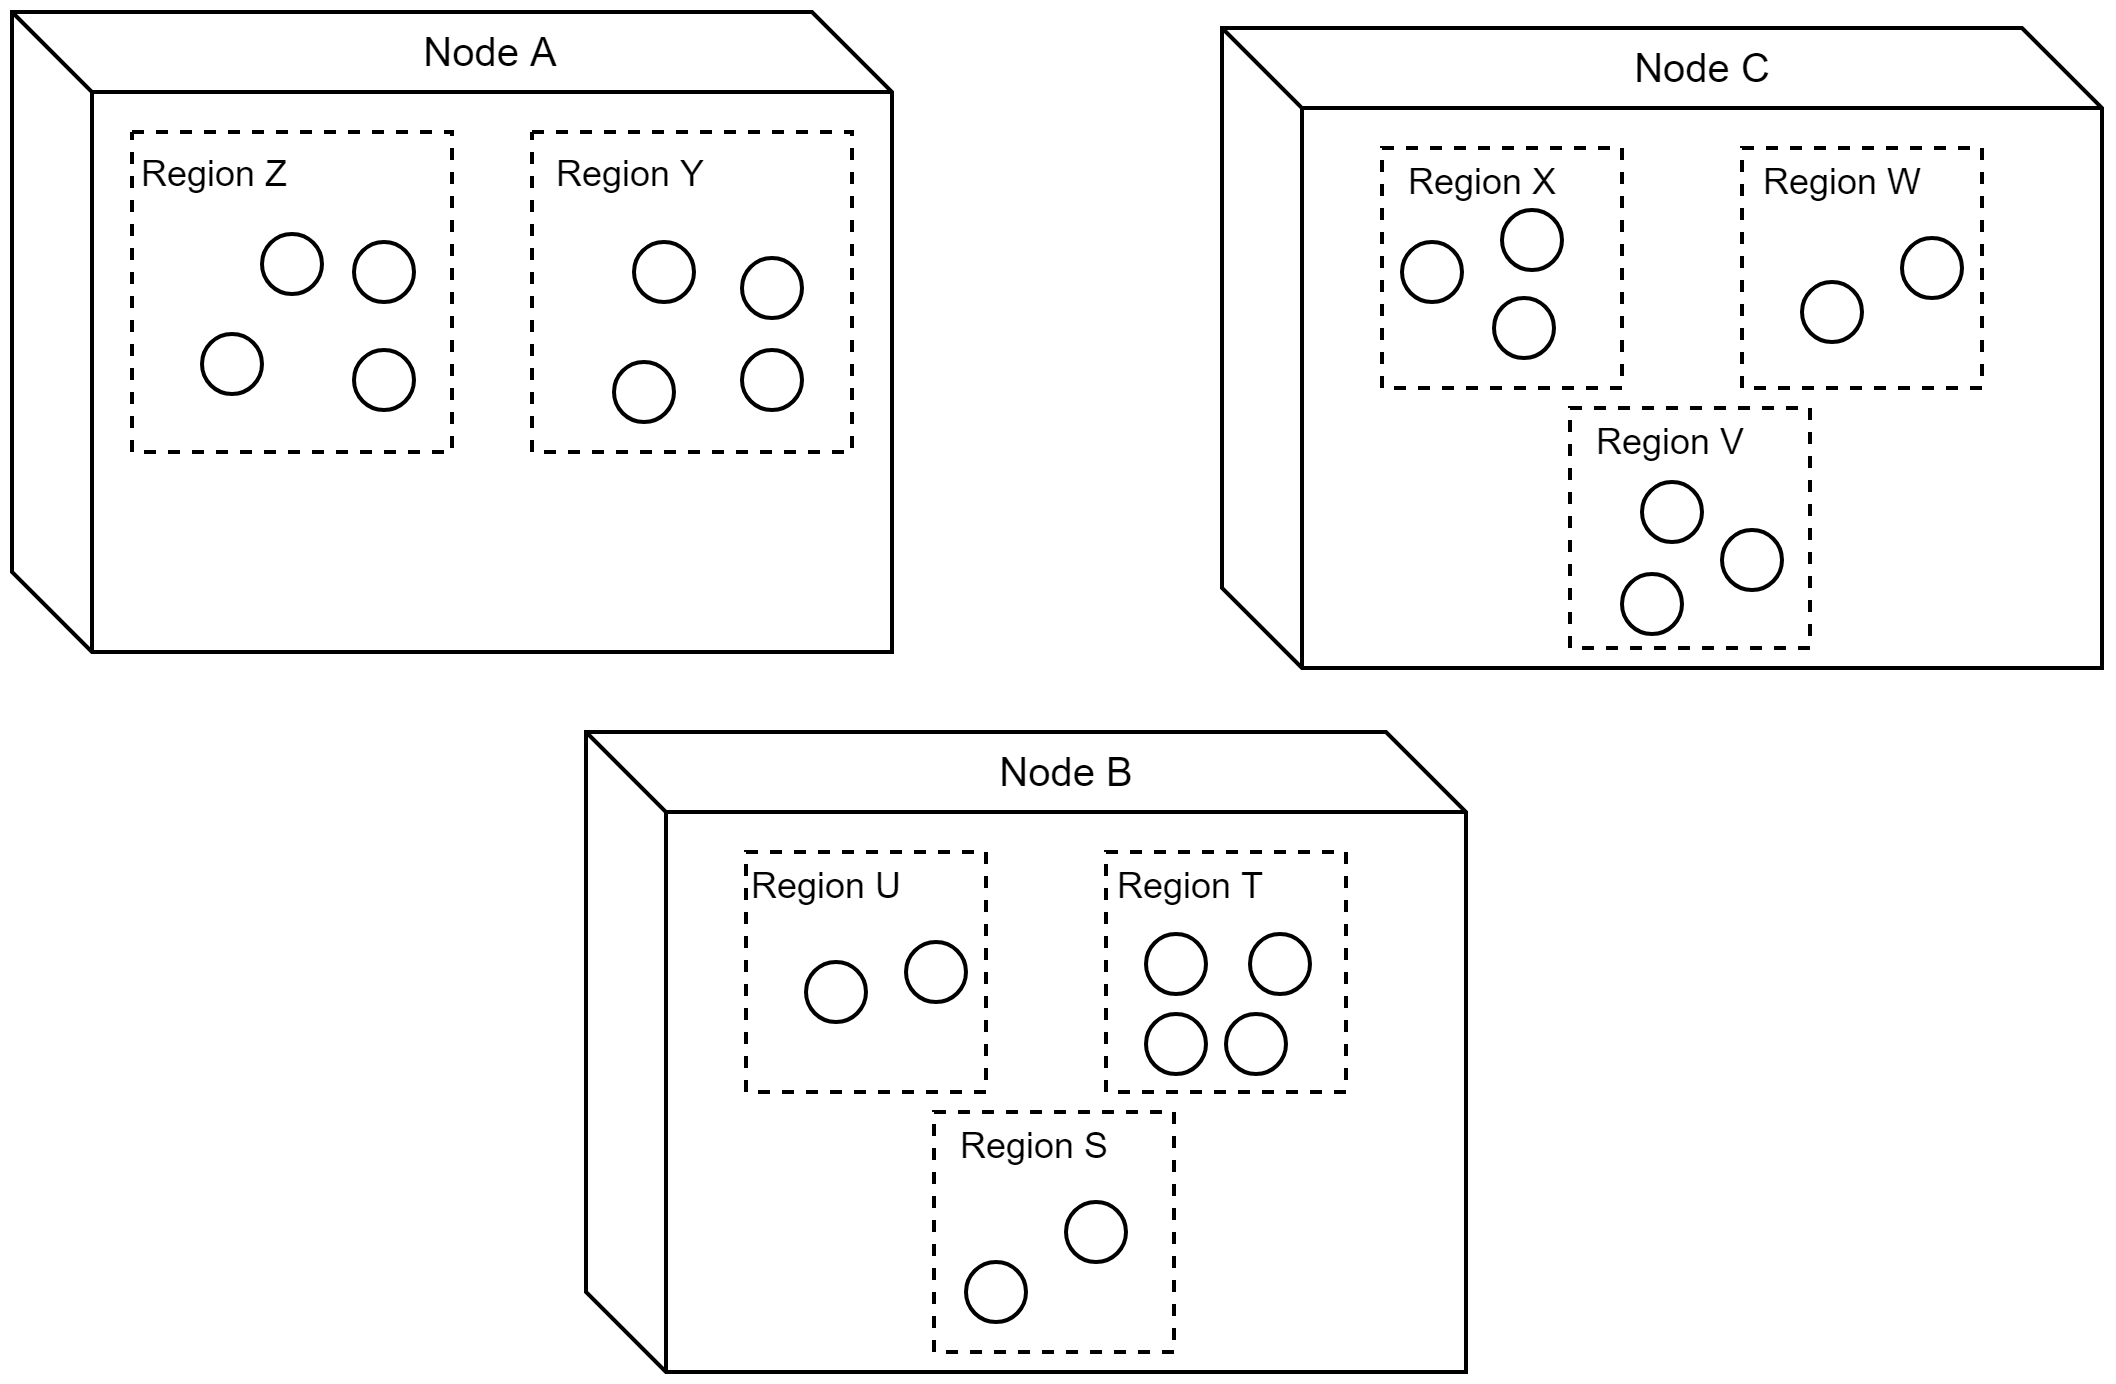
\includegraphics[width=0.8\linewidth]{gfx/implementation/Sharding}
  \caption{Verteilung von Entitäten in Shards, welche selbst wieder in \textit{Shard Groups} organisiert sind. Die Gruppen können zwischen den Nodes verteilt werden. }
  \label{fig:implementation:actorSharding}
\end{figure} 

Ein Grundprinzip von \textit{Sharding} ist die Unterteilung von Entitäten in unterschiedliche Gruppen, sogenannte \textit{Shards}. Dies wird in der \textit{Akka.net} Cluster Implementierung über die Zustellung von Nachrichten gelöst. Dazu werden Nachrichten nicht, wie bei Actor-Systemen, direkt an den Actor gesendet, sondern zuerst an einen Sharding Manager. Diese Nachrichten enthalten eine Identifikationsnummer der Entität, an die sie gerichtet sind. Der Manager interpretiert diese Nachricht und errechnet sich aus der Identifikationsnummer eine \textit{Shard} Identifikation. Anschließend prüft er, in welchem \textit{Shard Group} sich der \textit{Shard} befindet und welcher Node für diese Gruppe verantwortlich ist. Anschließend sendet er die Nachricht an den \textit{Shard Manager} auf dem entsprechenden Node. Hat sich dazwischen der \textit{Shard} auf einen anderen Node verschoben, kann der Node die Prüfung erneut durchführen und die Nachrichten an den neuen Zielort weiterleiten. Ist die gewünschte Entität am Node enthalten, stellt der dortige \textit{Shard Manger} die Nachricht an den entsprechenden Actor zu. \\
Für die Berechnung der \textit{Shard}-Identifikation auf Basis der Entitäts-Identifikation, wird in der Implementierung auf eine Hashfunktion zurückgegriffen. Der \textit{Shard Manager}, welcher die Nachricht an die zuständige \textit{Shard Region} weiterleiten soll, berechnet einen Integer Hashwert von der Entitäts-Identifikation. Diesen Wert Modulo der Anzahl an möglichen \textit{Shard Regions}, ergibt den \textit{Shard}, welcher für diese Entität zuständig ist. Die Anzahl der möglichen \textit{Shards} darf sich demnach zur Laufzeit des gesamten Clusters nicht verändern. Ansonsten würde durch die beschriebene Berechnungsfunktion neue \textit{Shards} entstehen und die Verteilung der Nachrichten schlägt fehlt. \\
Die Erzeugung von neuen Actoren in einem Shard wird durch Nachrichten an die noch nicht vorhandenen Actoren gestartet. Erhält ein \textit{Shard Manager} eine Nachricht an eine Entität, welche einem seiner \textit{Shards} zugeordnet werden kann und ist diese Entität noch nicht gestartet, so instanziiert der \textit{Shard Manager} einen neuen Actor. Dieser bekommt nun die Entitäts-Identifikation von der Nachricht zugewiesen.
